\clearpage

\section{SSPS for Apache ActiveMQ Artemis} \label{artemis}

In this section, we see various results of the prototypical implementation of SSPS for Apache ActiveMQ Artemis. First, we test for the difference in throughput with and without the SSPS. Then the CPU and memory utilization are measured. Finally, the failover scenario is tested.

\subsection{Throughput}
\subsubsection{Setup} \label{subsubsection:throughput_setup}

There are three entities involved in the setup. The publisher, subscriber and the broker (Apache ActiveMQ Artemis). All the three entities are running on a separate server instance having the following configuration on an open stack cluster.

\begin{itemize}
    \item \textbf{CPU:} Intel(R) Xeon(R) CPU E5-2630 v3 @ 2.40GHz
    \item \textbf{Memory:} 4 GB
    \item \textbf{OS:} Ubuntu xenial
\end{itemize}

We limit the bandwidth to 10KB/second using wondershaper \parencite{wondershaper} at the subscriber end to test the system for low bandwidth situation.

\subsubsection{Result}

The throughput is measured on the subscriber end. First, we examine the throughput without the SSPS on Apache ActiveMQ Artemis and then we monitor the throughput using SSPS on Apache ActiveMQ Artemis.

\paragraph{Throughput without SSPS} \mbox{} \\

Figure \ref{figures:throughput_wsdc} shows the throughput at the subscriber without the SSPS on Apache ActiveMQ Artemis. The average throughput is observed to be \textasciitilde14 messages/second.
\makeatletter
\setlength{\@fptop}{0pt}
\setlength{\@fpbot}{0pt}
\setlength{\intextsep}{20pt}
\makeatother

\begin{figure}[h!]
\centering
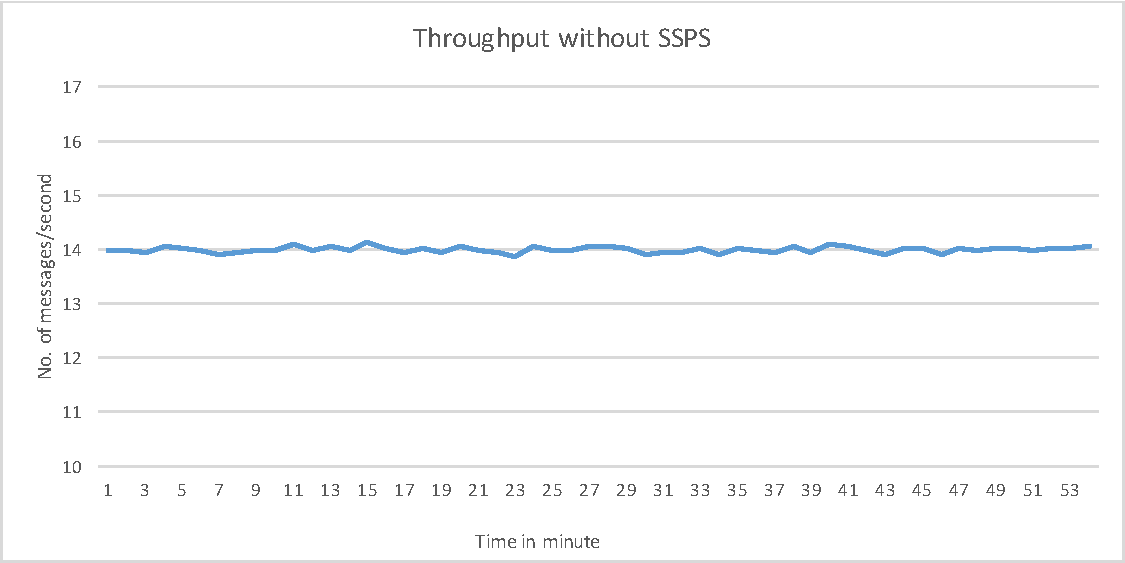
\includegraphics[scale=0.75]{throughput_wsdc.pdf}
\caption{Throughput without ssps}\label{figures:throughput_wsdc}
\end{figure}

\paragraph{Throughput with SSPS} \mbox{} \\

To use the SSPS on Apache ActiveMQ Artemis the interceptor needs to be configured in the \textit{broker.xml} configuration file \ref{subsubsection:in_interceptor}. Figure \ref{figures:throughput_sdc} shows the throughput at the subscriber with SSPS on Apache ActiveMQ Artemis. The average throughput is observed to be between 60 - 70 messages/second. 

\begin{figure}[h!]
\centering
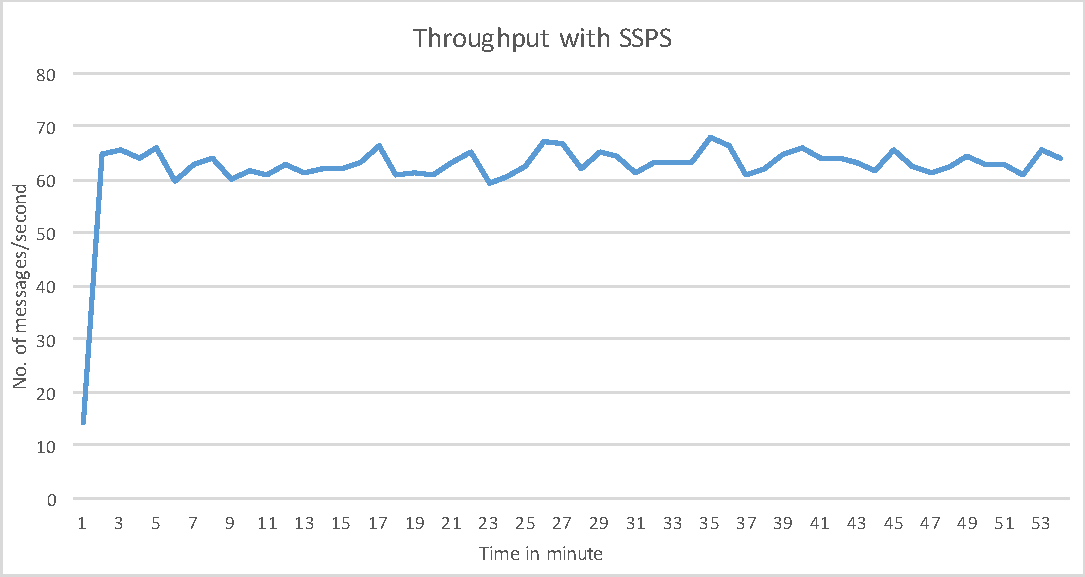
\includegraphics[scale=0.75]{throughput_sdc.pdf}
\caption{Throughput with ssps}\label{figures:throughput_sdc}
\end{figure}

The initial spike is because in SSPS model the first dictionary is sampled after 100 uncompressed messages and then made available. This happens only during the start of the system. Subsequent new clients do not suffer from these. Once the dictionary is available to the publisher and subscriber, there is a huge increase in the throughput at the subscriber end.

Figure \ref{figures:throughput_sdc_sec} shows the throughput for first few seconds when there is no dictionary sampled and made available. 

Figure \ref{figures:throughput_sdc2} shows the same result in a different way. The throughput is shown against timeline in seconds till the first dictionary is made available to the publisher and subscriber, and then the throughput is shown against timeline in minutes.

\begin{figure}[h!]
\centering
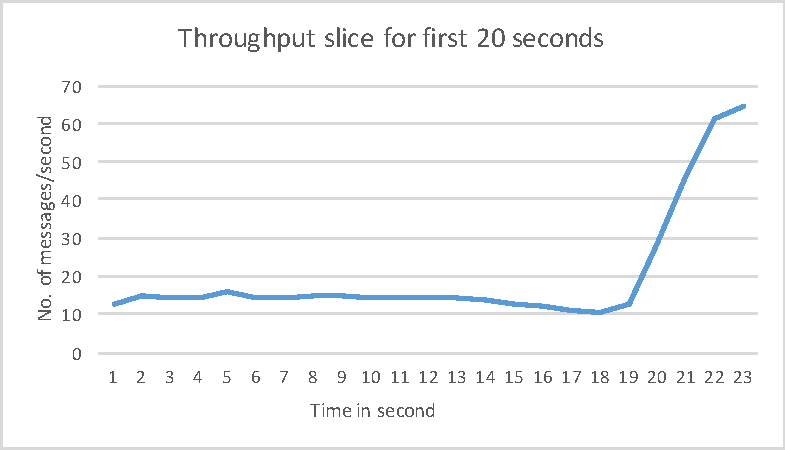
\includegraphics[scale=0.75]{throughput_sdc_sec.pdf}
\caption{Throughput slice for first 20 seconds}\label{figures:throughput_sdc_sec}
\end{figure}

\begin{figure}[h!]
\centering
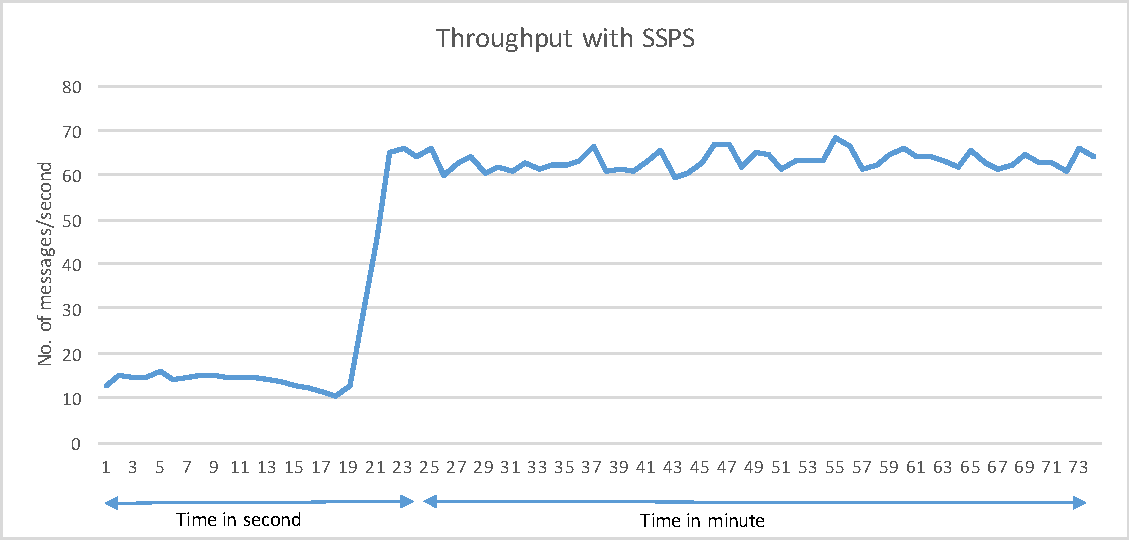
\includegraphics[scale=0.75]{throughput_sdc2.pdf}
\caption{Throughput with ssps}\label{figures:throughput_sdc2}
\end{figure}

\subsection{CPU and Memory Utilization} \label{cpu}

\subsubsection{Setup}

For measuring CPU and memory utilization for SSPS on Apache ActiveMQ Artemis the setup remains same as the setup for examining the throughput \ref{subsubsection:throughput_setup}. Except that we no longer need to limit the bandwidth on the subscriber end as the system under test is only the broker.

\subsubsection{Result}

The CPU utilization was measured in detail for various events such as sending and receiving uncompressed/compressed message to/from a queue, publishing dictionary and caching dictionary. Table \ref{table:cpu_utilization} shows the events and the corresponding CPU time in milliseconds.

\begin{table}[h!]
\centering
\caption{CPU utilization breakdown}
\label{table:cpu_utilization}
\begin{tabular}{ll}
    \toprule
    Event & Time (ms) \\
\midrule
    Sending uncompressed message to queue & 1.704772629 \\
    Receiving uncompressed message from queue & 2.329559 \\
    Sending compressed message to queue & 1.43901553 \\
    Receiving compressed message from queue    & 1.126042145 \\
    Sending dictionary to queue & 1.959809 \\
    Receiving dictionary from queue & 1.199765 \\
    Publishing dictionary & 122.71964 \\
    Caching dictionary & 4.558563 \\
\bottomrule
\end{tabular}
\end{table} 

The memory utilization while running SSPS on Apache ActiveMQ Artemis was observed to be \textasciitilde62 MB.

\subsection{Failover} \label{failover}

\subsubsection{Setup}

To test the failover scenario, a set up of an Apache ActiveMQ Artemis cluster having one live node and two backup nodes is used.

\subsubsection{Result}

The entire system normally runs on the live node. To test for failover, the live server is intentionally shut down abruptly after the dictionaries are published. The reason we need to wait at least for the first dictionary to be published is that the dictionary is made available for failover only when the dictionary is published and also if there is no dictionary available then the backup node cannot recover any dictionary and has to start the adaptive algorithm from the start.

Once we kill the live server, one among the two backup nodes takes over the live server and continues operating normally. The backup server, which is now the live server can handle the compressed messages as it now has the dictionary.



